\mysubsubsection{Lurking Behaviors and Initial Contact}\\
We explored lurking behavior and found that projects using Github as well as those using FAQ had longer lurking times. On the contrary, projects with formal onboarding material or {\it beginner bugs} identified had lower lurking time (see Table \ref{tab:lurking_time_regression}).

\begin{table}
\centering
\begin{tabular}{lccc}
Factor & $\beta$ & $\sigma(\beta)$ & significance \\
\hline 
Uses Github & 2.291 (1.170) & 0.480 & 0.071* \\ 
Has newcomer bugs & -0.309 (0.906) & -0.081 & 0.739 \\ 
Has a FAQ & 1.114 (0.834) & 0.290 & 0.203 \\ 
Has onboarding instructions & -1.372 (0.975) & -0.352 & 0.181 \\
\hline
Previous OCP experience & 0.104 (0.737) & 0.032 & 0.890 \\ 
\hline 
\end{tabular} 
\caption{Explaining lurking time. This model has rather good fitness (adj. $r^2$ 0.134); however other than the Github factor fail to achieve statistical significance. Without the beginner bug question, we can report significantly higher adj. $r^2$ in 0.185 without effects on other questions significance}
\label{tab:lurking_time_regression}
\end{table}

These results draw a mixed figure of the phenomena: having a FAQ might indicate complexity of the project or the level of institutionalization, which could explain our findings. However, the negative factor on {\it onboarding instructions} indicates that lurking might not be only about getting familiar with the community, rather also following and understanding the behaviors of the community, often explicated in on-boarding information.  We found it interesting that open collaboration project (OCP) development was clearly a non-significant factor and that the coefficient is approximately zero, therefore indicating that this control variable has no impact on lurking time.

Most participants answered that they {\bf have been lurking} prior to contacting the project, although the lurking period is widely spread\footnote{$21\%$ answered that the question is not applicable for them and their project.}.  


\begin{figure}[ht!]
\centering
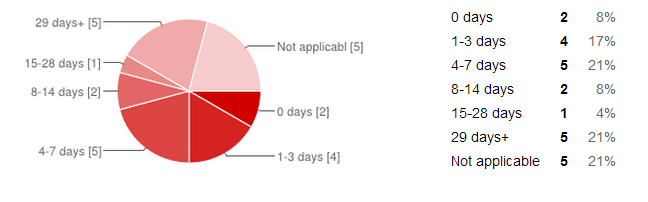
\includegraphics[width=120mm]{chapters/img/lurking_response.png}
\caption{Lurking Period}
\label{fig:lurking_period}
\end{figure}

About half of the people used private mail or through private email to get in contact with the community. While social networks might have an impact on open source software, social media was only used by one participant. This suggests that the impact of social media is still not well understood. In summary, personal email or to the mailing list remains the main initial communication means for joining.

\begin{figure}[ht!]
\centering
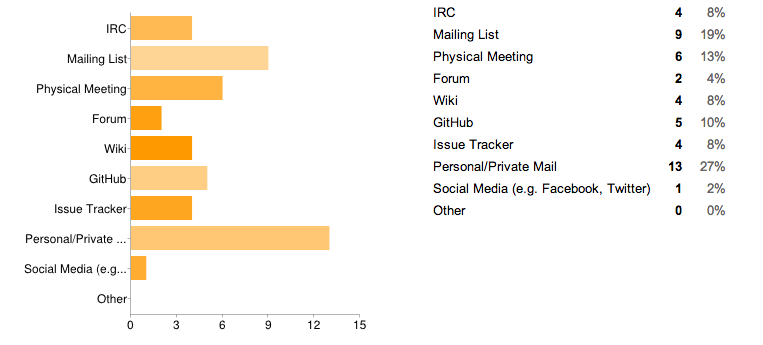
\includegraphics[width=120mm]{chapters/img/initial_contact.png}
\caption{Initial Contact}
\label{fig:initial_contact}
\end{figure}